\documentclass[aspectratio=169]{beamer}
\let\digamma\relax
\usepackage[romanfamily=casual,lucidasmallscale, nofontinfo]{lucimatx}
%\usepackage[romanfamily=bright-osf, stdmathdigits=true,lucidasmallscale, nofontinfo]{lucimatx}
\linespread{1.04} %  this value suits  scale=0.9  or lucidasmallscale
\usepackage{tikz}
\usepackage{pgfplots}
\pgfplotsset{compat=1.10}
\setbeamertemplate{navigation symbols}{}
\usefonttheme{professionalfonts,serif}

\begin{document}
\begin{frame}
    The function
    \[f(x,y) = \frac{xy^2}{x^2 + y^4}\]
    is a pretty simple function of two variables. 
    \pause
    \vspace{2\baselineskip}

    Even with such a simple function, though, we can see some interesting stuff
    going on when we look near the point of discontinuity, $(0,0)$.
\end{frame}
\begin{frame}[plain]
    \begin{columns}[T]
        \begin{column}{9.2cm}
            \centerline{%
            \begin{tikzpicture} 
                \begin{axis}[colormap/greenyellow,
                    axis lines=middle,
                    enlarge x limits=true,
                    enlarge y limits=true,
                    view={0}{90},
                    colorbar horizontal] 
                    \addplot3[surf,samples=80,domain=-1:1, shader=interp] {x*y^2/(x^2+y^4)}; 
                    \only<2->{\addplot3[red,very thick,samples=40,samples y=0, domain=-1:1] ({x^2},{x},{0});}
                    \only<3->{\addplot3[blue,very thick,samples=40,samples y=0, domain=-1:1] ({-x^2},{x},{0});}
                \end{axis} 
            \end{tikzpicture}
            }
        \end{column}
        \begin{column}{6.3cm}
            First look at the density plot of the function.\pause

            The areas that are bright yellow are where the function values are
            the highest. It looks like they form a parabola.\pause

            The areas that are the darkest green are where the function values
            are the lowest. Again, they seem to form a parabola.
        \end{column}
    \end{columns}
\end{frame}
\begin{frame}[plain]
    \begin{columns}[T]
        \begin{column}{9.2cm}
            \centerline{%
            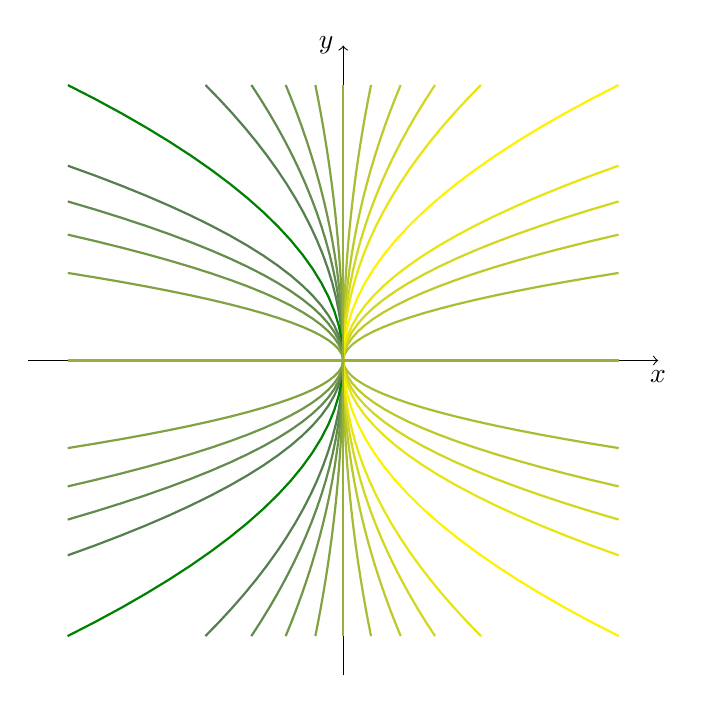
\begin{tikzpicture} 
                \def\scale{3.5}
                \colorlet{darkgreen}{green!50!black};
                \draw[thin,->] (-4,0) -- (4,0)node[below]{$x$};
                \draw[thin,->] (0,-4) -- (0,4)node[left]{$y$};
                \foreach \i in {-4,...,-1}{
                \pgfmathsetmacro{\k}{.1*\i};
                \pgfmathsetmacro{\coefa}{(1-sqrt(1-4*(\k)^2))/(2*\k)};
                \pgfmathsetmacro{\color}{10*(5+\i)};
                \draw[thick,color=yellow!\color!darkgreen] plot[domain=-1:1,samples=40] ({\scale*\coefa*(\x)^2},\scale*\x);
                }
                \draw[thick,color=darkgreen] plot[domain=-1:1,samples=40] ({-\scale*(\x)^2},\scale*\x);
                \begin{scope}
                    \clip (-\scale,-\scale) rectangle (\scale,\scale);
                    \foreach \i in {-4,...,-1}{
                    \pgfmathsetmacro{\k}{.1*\i};
                    \pgfmathsetmacro{\coefa}{(1+sqrt(1-4*(\k)^2))/(2*\k)};
                    \pgfmathsetmacro{\color}{10*(5+\i)};
                    \pgfmathsetmacro{\dom}{1/sqrt(-\coefa)}
                    \draw[thick,color=yellow!\color!darkgreen] plot[domain=-\dom:\dom,samples=40] ({\scale*\coefa*(\x)^2},\scale*\x);
                    }
                \end{scope}
                \foreach \i in {1,...,4}{
                \pgfmathsetmacro{\k}{.1*\i};
                \pgfmathsetmacro{\coefa}{(1-sqrt(1-4*(\k)^2))/(2*\k)};
                \pgfmathsetmacro{\color}{10*(5+\i)};
                \draw[thick,color=yellow!\color!darkgreen] plot[domain=-1:1,samples=40] ({\scale*\coefa*(\x)^2},\scale*\x);
                }
                \draw[thick,color=yellow] plot[domain=-1:1,samples=40] ({\scale*(\x)^2},\scale*\x);
                \begin{scope}
                    \clip (-\scale,-\scale) rectangle (\scale,\scale);
                    \foreach \i in {1,...,4}{
                    \pgfmathsetmacro{\k}{.1*\i};
                    \pgfmathsetmacro{\coefa}{(1+sqrt(1-4*(\k)^2))/(2*\k)};
                    \pgfmathsetmacro{\color}{10*(5+\i)};
                    \pgfmathsetmacro{\dom}{1/sqrt(\coefa)}
                    \draw[thick,color=yellow!\color!darkgreen] plot[domain=-\dom:\dom,samples=40] ({\scale*\coefa*(\x)^2},\scale*\x);
                    }
                \end{scope}
                \draw[thick,color=yellow!50!darkgreen] (-\scale,0) -- (\scale,0);
                \draw[thick,color=yellow!50!darkgreen] (0,-\scale) -- (0,\scale);
            \end{tikzpicture}
            }
        \end{column}
        \begin{column}{6.3cm}
            In fact, those two parabolas are the highest and the lowest
            contours on the contour plot of $f$.

            A contour plot of $f$ is shown here.

            We can see that the contours all seem to intersect at the point
            $(0,0)$.
        \end{column}
    \end{columns}
\end{frame}
\begin{frame}
    From all these plots we may begin to suspect that \[\lim_{(x,y)\to(0,0)}
    \frac{xy^2}{x^2+y^4}\]
    does not exist. As we approach the point $(0,0)$ along different level
    curves, we will get different limit.

    \uncover<2->{
    In fact, setting $x = ky^2$ and letting $y\to 0$, we get
    \begin{align*}
        \lim_{y\to 0} \frac{(ky^2)y^2}{(ky^2)^2 + y^4} =& \uncover<3->{\lim_{y\to 0}
        \frac{ky^4}{(k^2+1)y^4}}\\
        \uncover<4->{=& \lim_{y\to0} \frac{k}{k^2 + 1}} \uncover<5->{=  \frac{k}{k^2 + 1}}
    \end{align*}}
    \uncover<6->{For different values of $k$, we get different limits.}
\end{frame}
\begin{frame}
    It seems like we are able, when approaching the point $(0,0)$ on the
    $xy$-plane along different parabolas, to reach any point on the vertical
    segment connecting the points $(0,0,-1/2)$ and $(0,0,1/2)$.\pause

    In order to ``fix'' the discontinuity in the surface at $(x,y) = (0,0)$, we
    would have to add this whole vertical segment to the surface. It would then
    no longer be a graph of a function, though.\pause

    We see that not only is the function 
    \[f(x,y) = \frac{xy^2}{x^2 + y^4}\]
    discontinuous at $(0,0)$, this discontinuity is not fixable, and the
    function does not have a limit there.
\end{frame}
\end{document}
